\documentclass{article}

% Language setting
% Replace `english' with e.g. `spanish' to change the document language
\usepackage[english]{babel}

% Set page size and margins
% Replace `letterpaper' with`a4paper' for UK/EU standard size
\usepackage[letterpaper,top=2cm,bottom=2cm,left=3cm,right=3cm,marginparwidth=1.75cm]{geometry}

% Useful packages
\usepackage{amsmath}
\usepackage[colorlinks=true, allcolors=blue]{hyperref}

\usepackage{algorithm}
\usepackage{algpseudocode}
\usepackage{amsmath}
\usepackage{amsfonts,amssymb}
\usepackage[shortlabels]{enumitem}
\usepackage{setspace}
\usepackage{tikz}
\usepackage{bbm}
\usepackage{multicol}
\usepackage{cancel}
\usepackage{graphicx}
\usepackage{booktabs}
\usepackage{extarrows}

\title{CS229: Machine Learning}
\author{Junchuan Zhao}

\begin{document}
\setstretch{1.2} 
\maketitle

\begin{abstract}
This document includes my notes of CS229: Machine Learning.
\end{abstract}

\section{Lecture 2}
\subsection{Linear Regression}
Hypothesis: $h(x) = \sum\limits_{j=0}^n \theta_j x_j$ ($n$: number of features)

\noindent
Linear Regression: the hypothesis is the linear combination of the training dataset.

\noindent
Loss function (goal): $\min\limits_{\theta} \frac{1}{2} \sum\limits_{i=1}^m (h_{\theta}(x^i)-y^i)^2$

\noindent
Parameters: $\theta$, $m$, $n$, $x$, $y$

\subsection{Gradient Descent}
\subsubsection{Batch Gradient Descent}
Basic Ideas: start with some $\theta$, keep changing $\theta$ to reduce $J(\theta)$, repeat until convergent

\noindent
$\theta_j := \theta_j-\alpha\frac{\partial}{\partial \theta_j} J(\theta)$ ($\alpha$: learning rate)

\noindent
$\frac{\partial}{\partial \theta_j} J(\theta) = (h_\theta(x) - y) \cdot x_j$

\noindent
$\theta_j := \theta_j-\alpha \sum\limits_{i=1}^m (h_\theta(x)^i - y^i) \cdot x_j^i$ ($\alpha$: learning rate)

\noindent
Batch Gradient Descent: all the training data as a batch when optimizing the loss function.
(-): not good for large scale dataset, very expensive.

\subsubsection{Stochastic Gradient Descent}
\begin{algorithm}[h]
    \caption{Stochastic Gradient Descent}
  \label{alg::conjugateGradient}
  \begin{algorithmic}[1]
    \Require
    the parameter of $j^{th}$ feature
    \Ensure
    the updated parameter of $j^{th}$ feature
    \For {$i = 1$ to $m$}
        \State $\theta_j := \theta_j-\alpha \cdot (h_\theta(x)^i - y^i) \cdot x_j^i$;
    \EndFor
 
  \end{algorithmic}
\end{algorithm}

\noindent
stochastic gradient descent heads over to the global optimum.

\subsubsection{Total Equations}

A Total Equation for Stochastic Gradient Descent: $\nabla_{\theta}J(\theta) = \boldsymbol{0}$

\noindent
If A is square ($A \in \mathbb{R}_{n \times n}$)

Trace of A: $tr(A) = \sum\limits_{i}A_{ii}$

\noindent
Features of Trace:
\begin{itemize}[leftmargin=*, nosep]
    \item $tr(A) = tr(A^T)$
    \item $f(A) = tr(AB)$, $\nabla_{A}f(A) = B^T$
    \item $tr(AB) = tr(BA)$
    \item $tr(ABC) = tr(CAB)$
    \item $\nabla_{A}tr(AA^TC) = CA + C^TA$
\end{itemize}


~\\
\noindent
Loss Function: $\nabla_{\theta}J(\theta) = \frac{1}{2}(X\theta-y)^T(X\theta-y)$

\noindent
= $\frac{1}{2}(\theta^TX^T-y^T)(X\theta-y)$

\noindent
= $\frac{1}{2}(\theta^TX^TX\theta-\theta^TX^Ty-y^TX\theta)$

\noindent
= $X^TX\theta - X^Ty$

\noindent
Loss Function: $X^TX\theta - X^Ty = \boldsymbol{0}$ $\iff$ 
$X^TX\theta = X^Ty$

\noindent
$\theta = (X^TX)^{-1}X^Ty$

\section{Lecture 3}
\subsection{Locally Weighted Regression}
"Parametric" learning algorithm: fit fixed set of parameters ($\theta_i$) to data.

\noindent
"Non-parametric learning algorithm": amount of data/parameters you need to keep grows (linearly) with the size of data.

~\\
\noindent
Linear Regression: to evaluate $h$ at certain $x$

\noindent
Fit $\theta$ to minimize

$\frac{1}{2}\sum\limits_{i}(y^i-\theta^Tx^i)^2$, 

\noindent
return $\theta^Tx$


~\\
\noindent
Linear Regression: to evaluate $h$ at local region of $x$

\noindent
Fit $\theta$ to minimize

$\sum\limits_{i}w^i(y^i-\theta^Tx^i)^2$, 
where $w^i$ is a "weight function".

\noindent
common choice for $w^i$ is $w^i = e^{(-\frac{(x^i-x)^2}{2\tau^2})}$\\
If $\lvert x^i-x \rvert$ is small, then $w^i \approx 1$.\\
If $\lvert x^i-x \rvert$ is large, then $w^i \approx 0$.\\
$\tau$: bandwidth, control a larger or narrower window.

\subsection{Why Square Error?}

Assume $y^i = \theta^Tx^i + \epsilon^i$, where $\epsilon^i \sim  N(0, \sigma^2)$ models effects of random noise\\
$p(y^i|x^i;\theta) = \frac{1}{\sqrt{2\pi}\sigma}e^{-\frac{(y^i-\theta^Tx^i)^2}{2\sigma^2}}$\\
$\iff$ $y^i|x^i;\theta \sim N(\theta^Tx^i, \sigma^2)$\\

\noindent
Difference between Likelihood ($L$) and Probability ($P$): $L$ variess parameters, $P$ varies datapoints.
Assume the datapoints are IID,\\
The "likelihood" of $\theta$: $L(\theta) = p(\boldsymbol{y}|\boldsymbol{x};\theta)$
= $\prod\limits_{i=1}^m p(y^i|x^i;\theta)$\\
$l(\theta) = \log{\prod\limits_{i=1}^m\frac{1}{\sqrt{2\pi}\sigma}e^{(...)}}$
= $\sum\limits_{i=1}^m[\log{\frac{1}{\sqrt{2\pi}\sigma}} + \log{e^{(...)}}]$\\
= $m\log{\frac{1}{\sqrt{2\pi}\sigma}} - \sum\limits_{i=1}^m\frac{(y^i-\theta^Tx^i)^2}{2\sigma^2}$\\

\noindent
MLE: maximum likelihood estimation. Choose $\theta$ to maximize $L(\theta)$\\
i.e. choose $\theta$ to minimize $\frac{1}{2}\sum\limits_{i=1}^m(y^i-\theta^Tx^i)^2$, which is actually $J(\theta)$

\subsection{Classification}
Binary Classification: $y \in \{0,1\}$
\subsubsection{Logistic Regression}
We want $h_\theta(x) \in [0, 1]$, so we define\\
$h_\theta(x) = g(\theta^Tx) = \frac{1}{1 + e^{-\theta^Tx}}$\\
Sigmoid Function: $g(z) = \frac{1}{1 + e^{-z}}$\\
An important thing is that: the partial derivative of the sigmoid function is a \textbf{concave} function, which means it has the global maximum.
\begin{figure}[H]
	\centerline{
   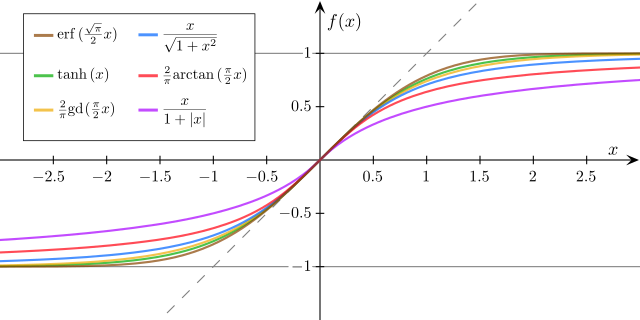
\includegraphics[width=0.5\textwidth]{Fig1.png}}
   \caption{The graph of sigmoid function.}
   \label{fig:example}
\end{figure}
\noindent
Different from Linear Regression $h_\theta(x) = \theta^Tx$, Logistic Regression is $h_\theta(x) = \frac{1}{1 + e^{-\theta^Tx}}$.\\
$p(y=1|x;\theta)=h_\theta(x)$, 
$p(y=0|x;\theta)=1-h_\theta(x)$\\
In sum, $p(y|x;\theta)=h_\theta(x)^y(1-h_\theta(x))^{1-y}$\\

\noindent
$L(\theta) = p(\boldsymbol{y}|\boldsymbol{x};\theta)$ = $\prod\limits_{i=1}^m h_\theta(x^i)^{y^i}(1-h_\theta(x^i))^{1-y^i}$\\
$l(\theta) = \log{(L(\theta))} = \sum\limits_{i=1}^m y^i\log{h_\theta(x^i)} + (1-y^i)\log{(1-h_\theta(x^i))}$\\
Choose $\theta$ to maximize $l(\theta)$, we use Batch gradient ascent.\\

\noindent
Batch Gradient Ascent:\\
\indent
$\theta_j := \theta_j + \alpha\frac{\partial}{\partial\theta_j}l(\theta)$\\
$\theta_j := \theta_j + \alpha\sum\limits_{i=1}^m(y^i-h_\theta(x^i))x_j^i$, same as the one in linear regression. (A larger category called generalized linear model (GLM))\\
Note: no \textbf{normal equation} for logistic regression solution.\\

\subsubsection{Newton's Method}
The basic idea: have some function $f$, we want to fit $\theta$, \textbf{s.t.} $f(\theta)=0$ $\iff$ want maximizing $l(\theta)$ $\iff$ want $l'(\theta)=0$\\
\begin{figure}[H]
	\centerline{
   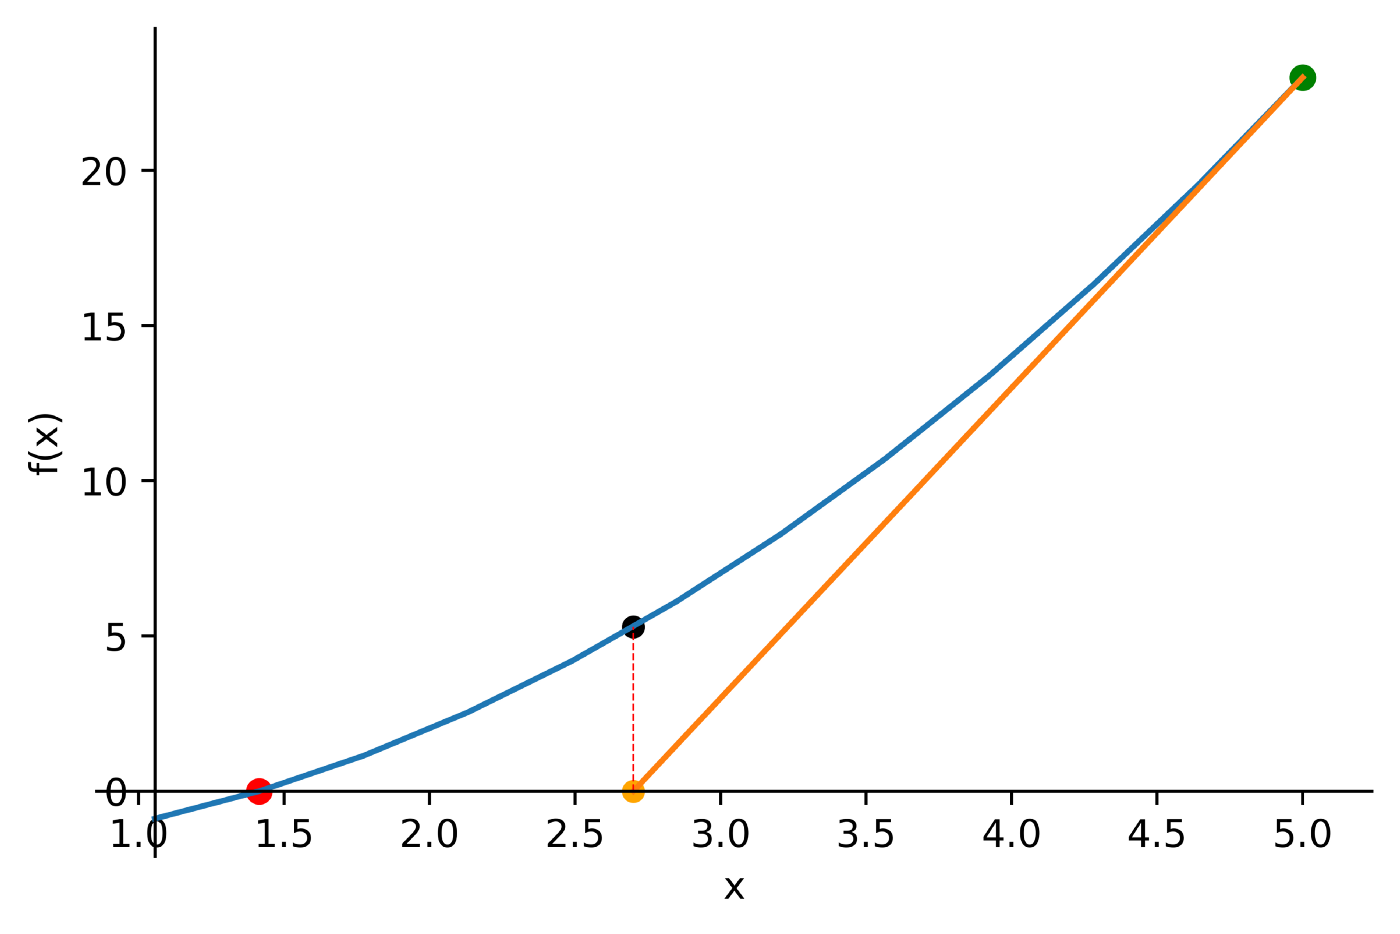
\includegraphics[width=0.5\textwidth]{Fig2.png}}
   \caption{Newton's Method.}
   \label{fig:example}
\end{figure}
\noindent
$\theta^{t+1} := \theta^{t} - \frac{f(\theta^t)}{f^{'}(\theta^t)}$, let $f(\theta) = l^{'}(\theta)$\\
$\theta^{t+1} := \theta^{t} - \frac{l^{'}(\theta^t)}{l^{''}(\theta^t)}$\\

\noindent
"\textbf{Quadratic convergent}": $0.01$ error $\longrightarrow$ $0.0001$ error $\longrightarrow$ $0.00000001$ error.\\

\noindent
When $\theta$ is a vector: ($\theta \in \mathbb{R}^{n+1}$)\\
\indent
$\theta^{t+1} := \theta^t + \alpha H^{-1}\nabla_\theta l(\theta)$\\
where 
$$
\nabla_\theta l(\theta) = 
\begin{bmatrix}
  \frac{\partial l}{\partial\theta_{00}} & \frac{\partial l}{\partial\theta_{01}} & \cdots & \frac{\partial l}{\partial\theta_{0n}} \\
  \frac{\partial l}{\partial\theta_{10}} & \frac{\partial l}{\partial\theta_{11}} & \cdots & \frac{\partial l}{\partial\theta_{1n}} \\
  \vdots & \vdots  & \ddots & \vdots \\
  \frac{\partial l}{\partial\theta_{n0}} & \frac{\partial l}{\partial\theta_{n1}} & \cdots & \frac{\partial l}{\partial\theta_{nn}} \\
\end{bmatrix}
$$
$H \in \mathbb{R}^{n+1 \times n+1}$ is the Hessian Matrix, $H_{ij} = \frac{\partial^2l}{\partial\theta_i\partial\theta_j}$\\
Note: If the dataset is large, the size of $H$ will be too large to compute.


\section{Lecture 4}
\subsection{Perceptron}
Binary step function: 
\begin{align}
  g(z)=
      \begin{cases}
      1 & z \geq 0 \\
      0 & z < 0 \\
      \end{cases}
\end{align}
\begin{figure}[H]
	\centerline{
   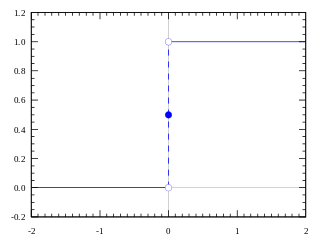
\includegraphics[width=0.5\textwidth]{Fig3.png}}
   \caption{The graph of binary step.}
   \label{fig:example}
\end{figure}
Batch Gradient Ascent: $\theta_j := \theta_j + \alpha(y^i-h_\theta(x^i))x_j^i$

\subsection{Exponential Family}
\subsubsection{Defination and Examples of Exponential Family}
Probability Density Function (PDF): $p(y;\eta) = b(y){\rm exp}[\eta^TT(y)-a(\eta)]$\\
$y$: data\\
$\eta$: natural parameter\\
$T(y)$: sufficient statistic\\
$b(y)$: base measure\\
$a(\eta)$: log partition\\

\noindent
Example 1:
Bernoulli (Binary Data): $p(y;\phi) = \phi^y(1-\phi)^{(1-y)}$\\
$\phi$ = probability of the event\\
$p(y;\phi) = {\rm exp}[y\log{(\frac{\phi}{1-\phi})} + \log{(1-\phi)}]$\\
$b(y) = 1$\\
$T(y) = y$\\
$\eta = \log{\frac{\phi}{1-\phi}}$ $\Rightarrow$ $\phi = \frac{1}{1 + e^{-\eta}}$ \\
$a(\eta) = -\log{(1-\phi)} = -\log{(1-\frac{1}{1 + e^{-\eta}})}$ = $\log{(1 + e^\eta)}$\\

\noindent
Example 2:
Gaussian (assume variance = 1): $p(y;\mu) = \frac{1}{\sqrt{2\pi}}e^{(-\frac{(y-\mu)^2}{2})}$
= $\frac{1}{\sqrt{2\pi}}e^{-\frac{y^2}{2}}{\rm exp}(\mu y-\frac{\mu^2}{2})$\\
$b(y) = \frac{1}{\sqrt{2\pi}}e^{-\frac{y^2}{2}}$\\
$T(y) = y$\\
$\eta = \mu$\\
$a(\eta) = \frac{\mu^2}{2} = \frac{\eta^2}{2}$

\subsubsection{Properties of Exponential Family}
\begin{itemize}[leftmargin=*, nosep]
  \item MLE w.r.t $\eta$ is concave, NLL is convex
  \item $E[y;\eta] = \frac{\partial}{\partial\eta}a(\eta)$
  \item $Var[y;\eta] = \frac{\partial^2}{\partial\eta^2}a(\eta)$
\end{itemize}
Real - Gaussian; Binary - Bernoulli; Count - Poisson; $\mathbb{R}^{+}$ - Gamma, Exponential; Distribution - Beta, Dirichlet (Bayesian).

\subsection{Generalized Linear Model (GLM)}
\subsubsection{GLM Assumptions}
Assumptions/Design Choices\\
(1) $y|x;\theta$ $\sim$ Exponential Family ($\eta$) \\
(2) $\eta = \theta^Tx$, $\theta \in \mathbb{R}^n$ and $x \in \mathbb{R}^n$ \\
(3) Test Time: output $h_\theta(x) = E[y|x;\theta]$
\subsubsection{GLM Pipeline}
\begin{figure}[H]
	\centerline{
   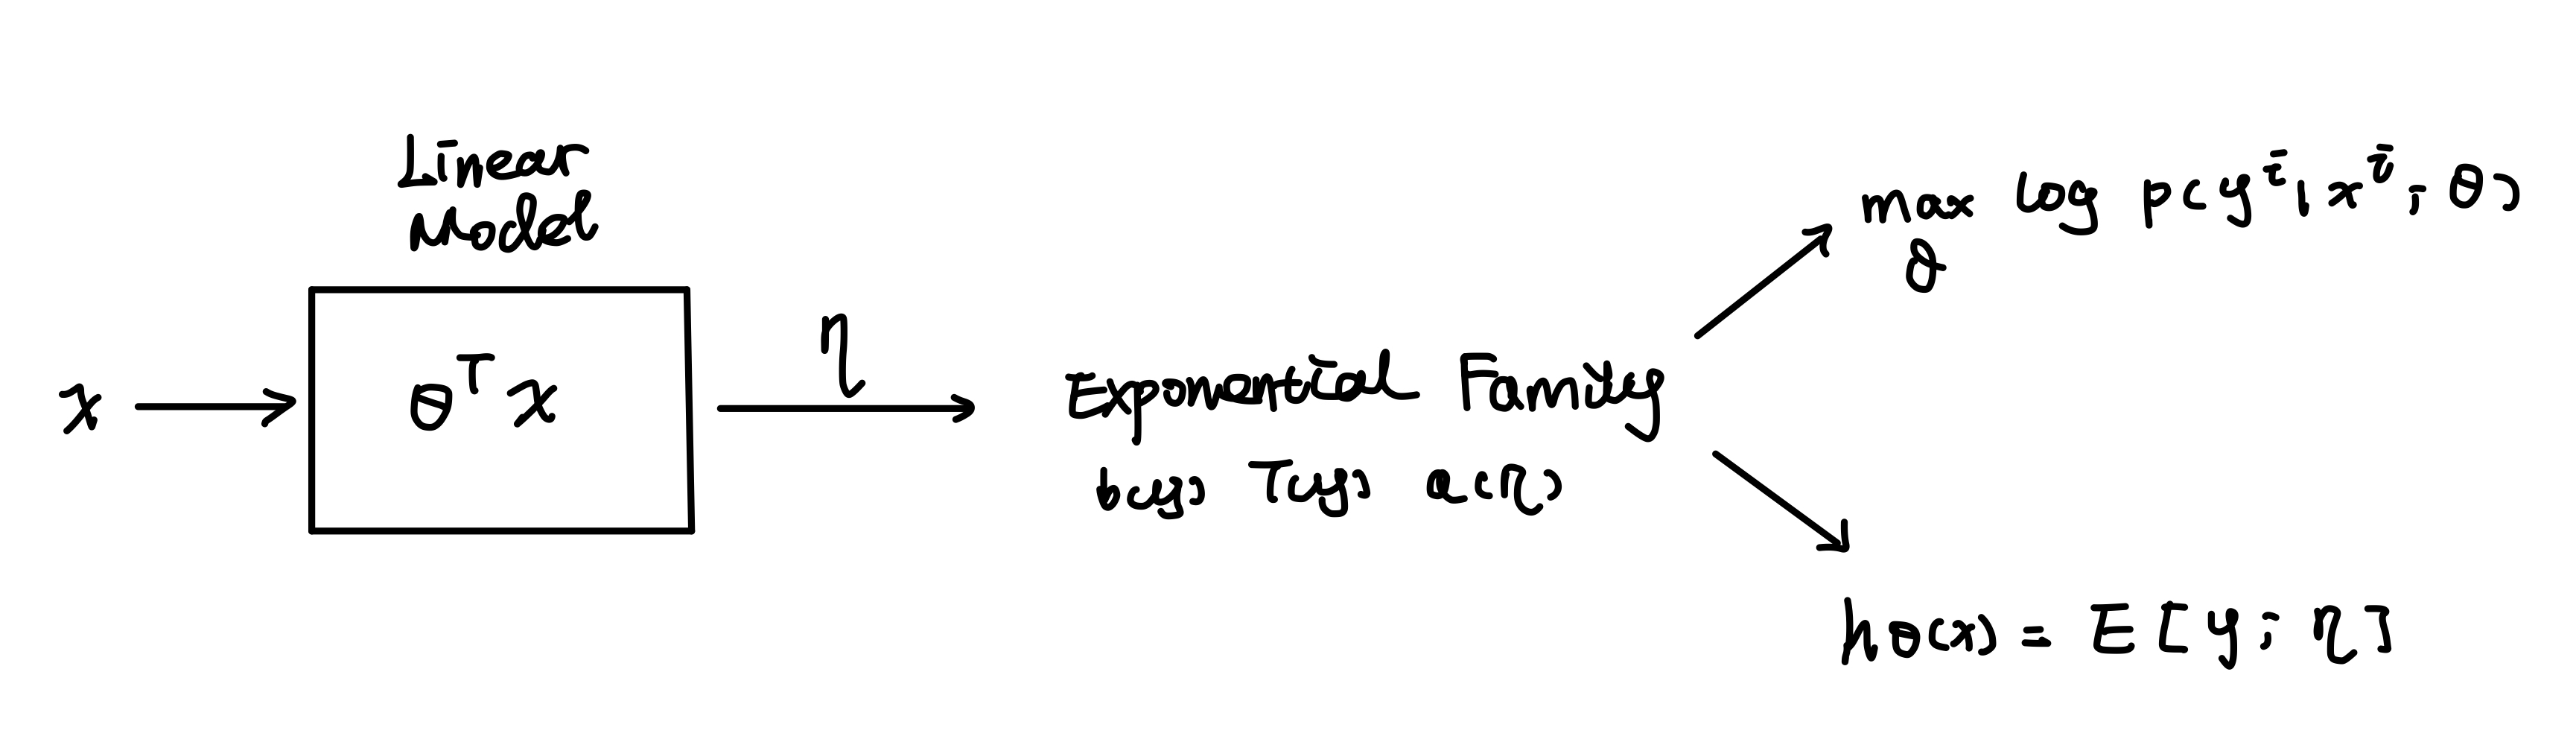
\includegraphics[width=0.7\textwidth]{Fig4.png}}
   \caption{The pipeline for GLM.}
   \label{fig:example}
\end{figure}
\subsubsection{GLM Training}
Learning Update Rule:
  $\theta_j := \theta_j + \alpha(y^i-h_\theta(x^i))x_j^i$\\

\noindent
Terminology:\\
$\eta$ - natural parameter\\
$g(\eta) = \mu = E(y;\eta)$ - canonical response function\\
$\eta = g^{-1}(\mu)$ - canonical link function\\

\noindent
Three parameterizations:\\
Model Param: $\theta$ (\textbf{Learn Parameters})\\
Natural Param: $\eta$ (Design Choice: $\theta^Tx$)\\
Canonical Param: $\phi$ - Bernoulli, $\mu$ $\sigma$ - Gaussian, $\lambda$ - Poisson (Canonical Response: $g(\cdot)$)

\subsubsection{Review Logistic Regression}
$h_\theta(x) = E[y|x;\theta] = \phi$ (the mean of the Bernoulli distribution)\\
$h_\theta(x) = \phi = \frac{1}{1+e^{-\eta}} = \frac{1}{1+e^{-\theta^Tx}}$

\subsection{Softmax Regression}
Task: multi-class Classification\\
$k$ - number of classes, $x^i \in \mathbb{R}^n$, Label $y^i \in \{0,1\}^k$ (one-hot vector)\\
Each class has its own parameters: $\theta_{class} \in \mathbb{R}^n$\\
$p(y=i|x;\theta) = \frac{e^{\theta_i^Tx}}{\sum_{j=1}^ke^{\theta_j^Tx}}$\\
$l(\theta) = \sum\limits_{i=1}^mlog\prod\limits_{l=1}^k(\frac{e^{\theta_l^Tx^i}}{\sum_{j=1}^ke^{\theta_j^Tx^i}})^{\{y^i = l\}}$


\section{Lecture 5}
\subsection{Discriminative v.s. Generative Learning Algorithms}
Discriminative: Learn $p(y|x)$ which is the mapping from x to y.\\

\noindent
Generative: Learn $p(x|y)$, $p(y)$ (class prior)\\
According to Bayes rule: $p(y|x) = \frac{p(x|y)p(y)}{p(x)}$, 
$p(x) = \sum\limits_{i=0}^kp(x|y=i)p(y=i)$

\subsection{Gaussian Discriminant Analysis (GDA)}
\subsubsection{Assumptions and Fundamental Knowledge}
Suppose $x \in \mathbb{R}^n$ (convention: drop $x_0=1$)\\
Assume $p(x|y)$ is Gaussian\\

Basic Knowledge for Multivariate Gaussian:\\
\indent
$z \sim N(\boldsymbol{\mu},\Sigma)$, ($z \in \mathbb{R}^n$)\\
\indent
$p(z) = \frac{1}{(2\pi)^{\frac{n}{2}}|\Sigma|^{\frac{1}{2}}}exp(-\frac{1}{2}(x-\boldsymbol{\mu})^T\Sigma^{-1}(x-\boldsymbol{\mu}))$
\indent
$E[z] = \boldsymbol{\mu}$\\
\indent
$Cov(z) = E[(z-\mu)(z-\mu)^T] = E_{zz^T}-E[z]{E[z]}^T$

\subsubsection{GDA model}
Parameters: $\boldsymbol{\mu_0}, \boldsymbol{\mu_1}, \Sigma$ (use same covariance matrix)\\
$p(x|y=0) = \frac{1}{(2\pi)^{\frac{n}{2}}|\Sigma|^{\frac{1}{2}}}exp(-\frac{1}{2}(x-\boldsymbol{\mu_0})^T\Sigma^{-1}(x-\boldsymbol{\mu_0}))$\\
$p(x|y=1) = \frac{1}{(2\pi)^{\frac{n}{2}}|\Sigma|^{\frac{1}{2}}}exp(-\frac{1}{2}(x-\boldsymbol{\mu_1})^T\Sigma^{-1}(x-\boldsymbol{\mu_1}))$\\
$p(y) = \phi^y(1-\phi)^y$ ($p(y=1)=\phi$)\\

\noindent
Training set: $\{(x^i, y^i)\}_{i=1}^m$\\
Joint Likelihood: $L(\phi,\boldsymbol{\mu_0}, \boldsymbol{\mu_1}, \Sigma) = \prod\limits_{i=1}^m p(x^i, y^i; \phi,\boldsymbol{\mu_0}, \boldsymbol{\mu_1}) 
= \prod\limits_{i=1}^m p(x^i|y^i)p(y^i)$\\
\indent\indent
Discriminative Learning (\textbf{Conditional Likelihood}): $\prod\limits_{i=1}^m p(y^i|x^i;\theta)$\\

\noindent
Maximize Likelihood Estimation (MLE):\\
$\max\limits_{\phi,\boldsymbol{\mu_0},\boldsymbol{\mu_1},\Sigma}l(\phi,\boldsymbol{\mu_0},\boldsymbol{\mu_1},\Sigma)$\\
Results of MLE:\\
$\phi = \frac{\sum\limits_{i=1}^m y^i}{m} = \frac{\sum\limits_{i=1}^m \mathbbm{1}\{y^i=1\}}{m}$ ($\mathbbm{1}: \mathbbm{1}\{{\rm true}\} = 1, \mathbbm{1}\{{\rm false}\} = 0$)\\
$\boldsymbol{\mu_0} = \frac{\sum\limits_{i=1}^m \mathbbm{1}\{y^i=0\}x^i}{\sum\limits_{i=1}^m \mathbbm{1}\{y^i=0\}} = \frac{{\rm sum\ of\ feature\ vectors\ for\ samples\ with\ y=0}}{{\rm number\ of\ samples\ with\ y=0}}$\\
$\boldsymbol{\mu_0} = \frac{\sum\limits_{i=1}^m \mathbbm{1}\{y^i=1\}x^i}{\sum\limits_{i=1}^m \mathbbm{1}\{y^i=1\}}$\\
$\Sigma = \frac{1}{m} \sum\limits_{i=1}^m(x^i-\mu_{y^i})(x^i-\mu_{y^i})^T$\\

\noindent
Prediction:\\
$\mathop{\arg\max}\limits_{y}p(y|x) = \mathop{\arg\max}\limits_{y}\frac{p(x|y)p(y)}{p(x)}$ ($p(x)$ is constant)\\
= $\mathop{\arg\max}p(x|y)p(y)$

\subsubsection{Compare GDA to Logistic Regression}
For fix parameters: $\phi,\boldsymbol{\mu_0}, \boldsymbol{\mu_1}, \Sigma$, 
plot $p(y|x; \phi,\boldsymbol{\mu_0},\boldsymbol{\mu_1},\Sigma)$ as a function of $x$.\\
By Bayes Rule: $p(y=1|x; \phi,\boldsymbol{\mu_0},\boldsymbol{\mu_1},\Sigma) = \frac{p(x|y=1;\boldsymbol{\mu_0},\boldsymbol{\mu_1},\Sigma)p(y=1;\phi)}{p(x; \phi,\boldsymbol{\mu_0},\boldsymbol{\mu_1},\Sigma)}$.\\
In the end, $p(y=1|x;\phi,\boldsymbol{\mu_0},\boldsymbol{\mu_1},\Sigma) = \frac{1}{1+exp(-\theta^Tx)}$, where $\theta$ is a function of $\phi,\boldsymbol{\mu_0},\boldsymbol{\mu_1},\Sigma$.\\

\noindent
The assumption of GDA $\Rightarrow$ $p(y=i|x) = \frac{1}{1 + e^{-\theta^Tx}}$\\
However, $p(y=i|x) = \frac{1}{1 + e^{-\theta^Tx}}$  $\bcancel{\Rightarrow}$ GDA assumptions.
\begin{table}[h]
  \begin{center}
  \begin{tabular}{cc}
    \toprule
    GDA & Logistic Regression \\
    \midrule
    stronger assumptions & weaker assumptions \\
    perform better when assumptions are correct & fine with all the scenarios (distributions) \\
    small dataset & large dataset \\
    computationally efficient & fits the era of the big data\\
    \bottomrule
  \end{tabular}
  \end{center}
  \caption{The comparison between GDA and Logistic Regression.}
  \label{tab:01}
\end{table}
\subsection{Naive Bayes}
For a spam email classification problem:\\
1. create a word dictionary (size $m$).\\
If represent $x$ by a binary feature vector, $x \in \{0,1\}^n$. ($x_i = \mathbbm{1}\{{\rm word\ i\ appears\ in\ email}\}$)\\
\indent
This cause $2^n$  possible values of x, which is not possible for large dictionary.\\
2. Assume \textbf{$x_i$'s are conditionally independent given y}, which means\\
\indent
$p(x_1, ..., x_{10000}|y) = p(x_1|y)p(x_2|x_1,y)p(x_3|x_1,x_2,y) ... p(x_{10000}|...,y)$\\
\indent
$\xlongequal{{\rm assume}}$ $p(x_1|y)p(x_2|y)...p(x_{10000}|y)$
= $\prod\limits_{i=1}^np(x_i|y)$\\

\noindent
Parameters:\\
$\phi_{j|y=1} = p(x_j=1|y=1)$\\
$\phi_{j|y=0} = p(x_j=1|y=0)$\\
$\phi_{y} = p(y=1)$\\

\noindent
Joint Likelihood: 
$L(\phi_i, \phi_{j|y}) = \prod\limits_{i=1}^mp(x^i,y^i;\phi_j,\phi_{j|y})$\\
MLE results:
$\phi_y = \frac{\sum\limits_{i=1}^m\mathbbm{1}\{y^i=1\}}{m}$\\
$\phi_{j|y=1} = \frac{\sum\limits_{i=1}^m\mathbbm{1}\{x_j^i=1,y^i=1\}}{\sum\limits_{i=1}^m\mathbbm{1}\{y^i=1\}}$\\
$\phi_{j|y=0} = \frac{\sum\limits_{i=1}^m\mathbbm{1}\{x_j^i=1,y^i=0\}}{\sum\limits_{i=1}^m\mathbbm{1}\{y^i=0\}}$\\

\noindent
At prediction time:\\
$p(y=1|x) = \frac{p(x|y=1)p(y=1)}{p(x|y=1)p(y=1)+p(x|y=0)p(y=0)}$\\
Problem: when a word does not exist -- $\frac{0}{0}$

\section{Lecture 6}
\subsection{Laplace Smoothing}
$x \in \{1, ..., k\}$, estimate $p(x=j) = \frac{\sum\limits_{j=1}^m\mathbbm{1}\{x^i=j\} {\color{red} + 1}}{m + {\color{red} + k}}$\\
$\phi_{j|y=0} = \frac{\sum\limits_{i=1}^m\mathbbm{1}\{x_j^i=1,y^i=0\} {\color{red} + 1}}{\sum\limits_{i=1}^m\mathbbm{1}\{y^i=0\}{\color{red} + 2}}$

\subsection{Multinomial Event Model}
$x \in 
\begin{bmatrix}
600\\
800\\
1600\\
6200\\
\end{bmatrix}$, $x \in \mathbb{R}^n$\\
$x_j \in \{1, 2, ..., 10000\}$, $n$ = length of email, $m$ = number of emails\\
Parameters: $\phi_y=p(y=1), \phi_{k|y=0} = p(x_j=k|y=0), \phi_{k|y=1} = p(x_j=k|y=1)$\\

\noindent
MLE results: $\phi_{k|y=0} = \frac{\sum\limits_{i=1}^m (\mathbbm{1}\{y^i=0\}\sum\limits_{j=1}^{n_i} \mathbbm{1}\{x_j^i=k\})}{\sum\limits_{i=1}^m \mathbbm{1}\{y^i=0\}n_i}$\\
$\xlongequal{{\rm laplace\ smoothing}}$ = $\frac{\sum\limits_{i=1}^m (\mathbbm{1}\{y^i=0\}\sum\limits_{j=1}^{n_i} \mathbbm{1}\{x_j^i=k\}) + 1}{\sum\limits_{i=1}^m \mathbbm{1}\{y^i=0\}n_i + 10000}$\\

\noindent
The advantages for GDA and Naive Bayes: quick to train, non-iterative.

\subsection{Support Vector Machines {SVM}}
SVM helps to find non-linear boundaries for classification problems.

\subsubsection{Optimal Margin Classifier}
Functional Margin: how confidentaly and accurately to classify an example.\\
\indent
Logistic Regression: $h_\theta(x) = g(\theta^Tx)$, predict $1$ if $\theta^Tx \geq 0$ and $0$ otherwise.\\
\indent
We want if $y^i=1$, hope that $\theta^Tx^i \gg 0$ and $0$ when $\theta^Tx^i \ll 0$. -- correct or confident prediction.\\

\noindent
Notation: Labels $y \in \{-1, +1\}$, 
\begin{align}
  g(z)=
      \begin{cases}
      1 & z \geq 0 \\
      -1 & z < 0 \\
      \end{cases}
\end{align}
$h_{W,b}(x) = g(W^Tx+b)$, $W \in \mathbb{R}^n$ and $b \in \mathbb{R}$. (Compare to Logistic Regression, $b$ is $\theta_0$)\\

\noindent
Functional Margin of hyperplane defined by ($W$, $b$) w.r.t $(x^i, y^i)$:\\
\indent $\hat{\gamma}^i = y^i(W^Tx^i+b)$, we want $\gamma^i \gg 0$\\
Funtional Margine w.r.t training set: $\hat{\gamma} = \min\limits_{i}\hat{\gamma}^i$, $i = 1, ..., m$\\
Rescaling the parameters: $(W,b)$ $\rightarrow$ $(\frac{W}{\Vert W \Vert}, \frac{b}{\Vert W \Vert})$\\

\noindent
Geometric Margin: the distance from the data point to the hyperplane.
\begin{figure}[H]
	\centerline{
   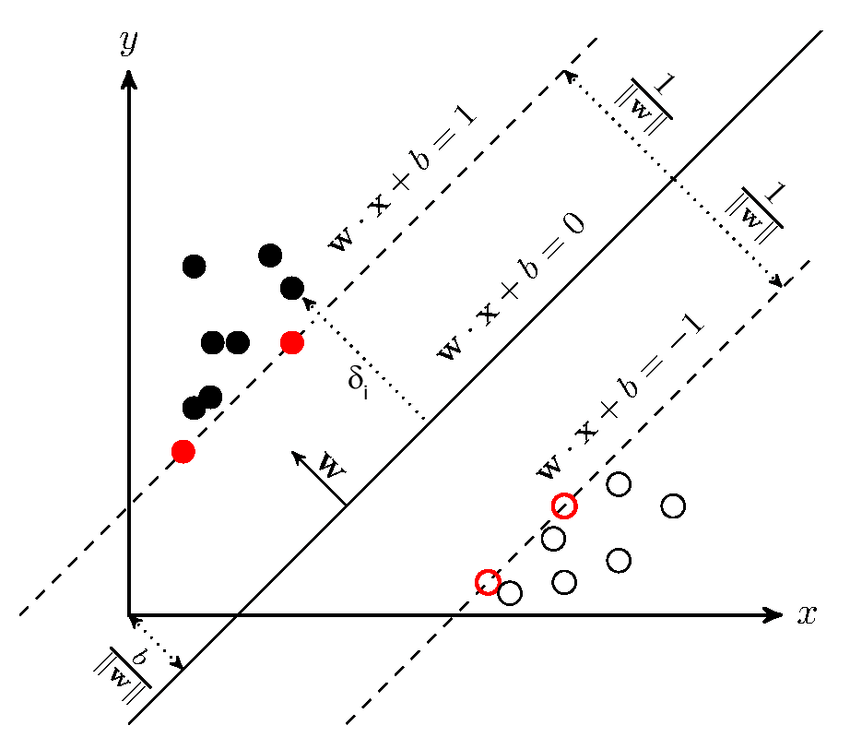
\includegraphics[width=0.6\textwidth]{Fig5.png}}
   \caption{Geometric Margin.}
   \label{fig:example}
\end{figure}
Geometric Margin of hyperplane ($W$,$b$) w.r.t ($x^i$,$y^i$):\\
\indent
$\gamma^i = \frac{y^i(W^Tx^i+b)}{\Vert W \Vert}$\\
Geometric Margin w.r.t training set: $\gamma = \min\limits_{i}\gamma^i$\\
The relationship between geometric and functional margin: $\gamma^i = \frac{\hat{\gamma}^i}{\Vert W \Vert}$\\
$\hat{\gamma}$ is functional margin; $\gamma$ is geometric margin.\\

\noindent
Optimal margin classifier: choose $w$, $b$ to maximize $\gamma$:\\
\indent
$\max\limits_{\gamma,w,b}\gamma$ s.t. $\frac{y^i(W^Tx^i+b)}{\Vert W \Vert} \geq \gamma$, ($i = 1, ..., m$.) 
$\Rightarrow$ $\min\limits_{w,b} {\Vert W \Vert}^2$ s.t. $y^i(W^Tx^i+b) \geq 1 $

\end{document}